\section{Recursions}

\subsection{Variables}

$S^1, S^2$ target and query sequences\\
$i_1, j_1, i_2, j_2$ interaction boundaries\\
$si_1, sj_1, si_2, sj_2$ seed boundaries\\
$N$ the maximum interaction length $(\sim 150)$\\
$M$ the maximum loop length $(\sim 15)$

\subsection{Recursion 1 ($n^{4}$ space + time)}

\begin{figure}[H]
	\centering
	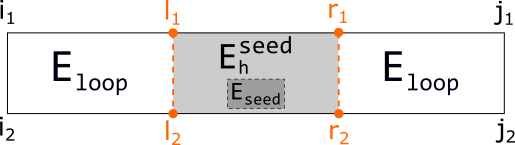
\includegraphics[scale=0.65]{seedenergy.png}
\end{figure}

Initialization:\\

\begin{equation*}
E_h(\substack{si_1,sj_1\\si_2,sj_2}) = E_{seed} + ED_{1}(si_{1}, sj_{1}) + ED_{2}(si_{2},sj_{2})
\end{equation*}

\begin{equation*}
\underset{{\substack{si_1 < i_{1} <= j_{1} < sj_{1}\\si_2 < i_{2} <= j_{2} < sj_{2}}}}{\forall} E_h(\substack{i_1,j_1\\i_2,j_2}) = \infty
\end{equation*}

Recursion:\\

\begin{equation*}
\substack{
  \underset{\substack{si_{1}-N <= i_{1} <= si_{1}\\si_{2}-N <= i_{2} <= si_{2}}}{\forall}\\
  \underset{\substack{sj_{1} <= j_{1} <= sj_{1}+N\\sj_{2} <= j_{2} <= sj_{2}+N}}{\forall}
}
E_h(\substack{i_1,j_1\\i_2,j_2}) = \begin{cases}
  \infty\\
  \quad\text{: if } \text{ no matching base pair }\\
  \infty\\
  \quad\text{: if } j_{1} - i_{1} > N \text{ oder } j_{2} - j_{1} > N\\
  \min\limits_{\substack{i_{1} < l_{1} <= r_{1} < j_{1}\\i_{2} < l_{2} <= r_{2} < j_{2}\\l_{1} - i_{1} < M\\j_{1}-r_{1} < M\\l_{2} - i_{2} < M\\j_{2}-r_{2} < M}}
  \begin{pmatrix}
	E_{loop}(\substack{i_1,l_1\\i_2,l_2}) + E_h(\substack{l_1,r_1\\l_2,r_2}) + E_{loop}(\substack{r_1,j_1\\r_2,j_2})
  \end{pmatrix}\\
  \quad\text{: otherwise.}\\
  
\end{cases}
\end{equation*}

\clearpage

\subsection{Recursion 2 ($n^{2}$ space + $n^{4}$ time)}

\begin{figure}[H]
	\centering
	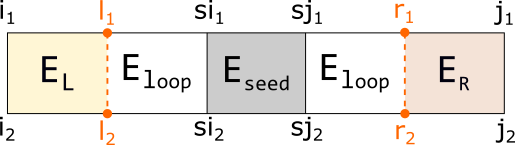
\includegraphics[scale=0.65]{seedenergy2.png}
\end{figure}

Recursion:\\

\begin{equation*}
E_h(\substack{i_1,j_1\\i_2,j_2}) = \underset{\substack{j_{1} - i_{1} < N\\j_{2} - i_{2} < N}}{\min}(ED_{1} + ED_{2} + E_{seed} + E_{L} + E_{R})
\end{equation*}

\begin{equation*}
\underset{i1, i2}{\forall}
E_L(\substack{i_1\\i_2}) = \begin{cases}
\infty\\
\quad\text{: if } \text{ no matching base pair }\\
\min\limits_{\substack{l1, l2}}
\begin{pmatrix}
E_L(\substack{l_1\\l_2}) + E_{loop}(\substack{i_1,l_1\\i_2,l_2})
\end{pmatrix}\\
\quad\text{: otherwise.}\\

\end{cases}
\end{equation*}

\begin{equation*}
\underset{j1, j2}{\forall}
E_R(\substack{j_1\\j_2}) = \begin{cases}
\infty\\
\quad\text{: if } \text{ no matching base pair }\\
\min\limits_{\substack{r1, r2}}
\begin{pmatrix}
E_{loop}(\substack{r_1,j_1\\r_2,j_2}) + E_R(\substack{r_1\\r_2})
\end{pmatrix}\\
\quad\text{: otherwise.}\\

\end{cases}
\end{equation*}

